% This section uses TikZ figures. Ensure the preamble includes: \usepackage{tikz}

\section{Worked Examples and Visual Case Studies}

The earlier sections of this chapter introduced the main generative paradigms one by one.
A reader may understand each paradigm locally and still not yet have the comparative judgment that matters most in practice.
This section therefore slows down and works through a small set of low-dimensional examples.
The point is not to showcase large-scale engineering success.
The point is to see, on the same kinds of toy problems, how different generative models represent uncertainty, hidden structure, and generation itself.

\medskip

Whenever possible, we use either the same target distribution or closely related toy distributions:
a bimodal one-dimensional dataset, a low-dimensional latent line between two examples, a two-dimensional warped density, and an iterative denoising path from noise back to structure.
These examples are intentionally simple enough that one can inspect the equations and the pictures at the same time.

\subsection*{Case study 1: Gaussian mixture and EM walk-through}

A Gaussian mixture model is still the cleanest worked example of latent-variable generative modeling.
Suppose the observed one-dimensional data are
\[
\mathcal{D}=\{-2.2,-1.8,2.1,2.4\},
\]
and consider a two-component Gaussian mixture with fixed variance $\sigma^2=1$:
\[
p_\theta(x)=\pi_1\,\mathcal{N}(x\mid \mu_1,1)+\pi_2\,\mathcal{N}(x\mid \mu_2,1),
\qquad \pi_1+\pi_2=1.
\]
The latent variable $z_i\in\{1,2\}$ indicates which component generated $x_i$.

We initialize
\[
\pi_1^{(0)}=\pi_2^{(0)}=\tfrac12,
\qquad
\mu_1^{(0)}=-1,
\qquad
\mu_2^{(0)}=1.
\]
The E-step computes responsibilities
\[
r_{ik}
=
\mathbb{P}(z_i=k\mid x_i,\theta^{(0)})
=
\frac{\pi_k^{(0)}\,\mathcal{N}(x_i\mid \mu_k^{(0)},1)}{\sum_{j=1}^2 \pi_j^{(0)}\,\mathcal{N}(x_i\mid \mu_j^{(0)},1)}.
\]
Because the data are well separated, the responsibilities are already nearly hard assignments:
\[
r_{11}\approx 0.992,\quad r_{21}\approx 0.973,
\qquad
r_{31}\approx 0.043,\quad r_{41}\approx 0.032,
\]
so points near $-2$ are assigned mostly to component 1 and points near $2$ mostly to component 2.

The M-step updates mixture weights and means:
\[
\pi_k^{(1)}=\frac{1}{n}\sum_{i=1}^n r_{ik},
\qquad
\mu_k^{(1)}=\frac{\sum_i r_{ik}x_i}{\sum_i r_{ik}}.
\]
With the approximate responsibilities above,
\[
\pi_1^{(1)}\approx 0.510,
\qquad
\pi_2^{(1)}\approx 0.490,
\]
and
\[
\mu_1^{(1)}
\approx
\frac{0.992(-2.2)+0.973(-1.8)+0.043(2.1)+0.032(2.4)}{0.992+0.973+0.043+0.032}
\approx -1.84,
\]
\[
\mu_2^{(1)}
\approx
\frac{0.008(-2.2)+0.027(-1.8)+0.957(2.1)+0.968(2.4)}{0.008+0.027+0.957+0.968}
\approx 2.15.
\]
After just one iteration, the parameters move toward the visible cluster centers.
The example is pedagogically important because every step can be interpreted:
soft latent assignment simplifies the optimization of an otherwise nonconvex incomplete-data likelihood.

\begin{figure}[h]
\centering
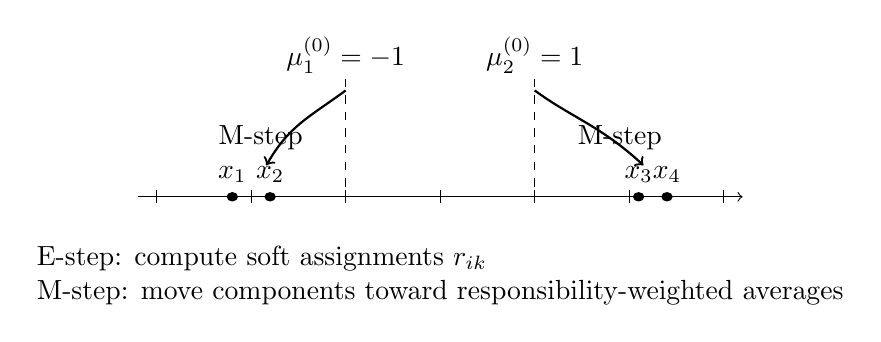
\begin{tikzpicture}[x=1.2cm,y=1cm]
    \draw[->] (-3.2,0) -- (3.2,0);
    \foreach \x in {-3,-2,-1,0,1,2,3} {\draw (\x,0.08) -- (\x,-0.08);}    
    \node at (-2.2,0.28) {$x_1$};
    \node at (-1.8,0.28) {$x_2$};
    \node at (2.1,0.28) {$x_3$};
    \node at (2.4,0.28) {$x_4$};
    \fill (-2.2,0) circle (0.06);
    \fill (-1.8,0) circle (0.06);
    \fill (2.1,0) circle (0.06);
    \fill (2.4,0) circle (0.06);

    \draw[dashed] (-1,1.5) -- (-1,0.1);
    \draw[dashed] (1,1.5) -- (1,0.1);
    \node at (-1,1.8) {$\mu_1^{(0)}=-1$};
    \node at (1,1.8) {$\mu_2^{(0)}=1$};

    \draw[->,thick] (-1,1.35) .. controls (-1.4,1.0) and (-1.6,0.9) .. (-1.84,0.4);
    \draw[->,thick] (1,1.35) .. controls (1.4,1.0) and (1.7,0.9) .. (2.15,0.4);
    \node at (-1.9,0.75) {M-step};
    \node at (1.9,0.75) {M-step};

    \node[align=left] at (0,-1.0) {E-step: compute soft assignments $r_{ik}$\\M-step: move components toward responsibility-weighted averages};
\end{tikzpicture}
\caption{A one-iteration EM walk-through for a two-component Gaussian mixture. The latent assignment variables are not observed, but the E-step estimates them and the M-step refits the component parameters.}
\label{fig:emwalkthrough}
\end{figure}

\subsection*{Case study 2: VAE latent interpolation sketch}

A variational autoencoder gives a different generative picture.
Instead of assigning each point to one of finitely many latent components, it learns a continuous latent coordinate $z$ together with a decoder $p_\theta(x\mid z)$.
A simple way to visualize what the model has learned is to encode two data points, interpolate in latent space, and decode back.

Suppose two observations $x^{(a)}$ and $x^{(b)}$ are encoded to approximate posterior means
\[
\mu_\phi(x^{(a)})=-1.2,
\qquad
\mu_\phi(x^{(b)})=1.4,
\]
in a one-dimensional latent space.
For interpolation parameter $\lambda\in[0,1]$, define
\[
z_\lambda=(1-\lambda)(-1.2)+\lambda(1.4).
\]
If the decoder mean is approximately linear near this path, say
\[
\mathbb{E}[x\mid z]\approx 2z,
\]
then the decoded means along the path are
\[
-2.4,\,-1.1,\,0.2,\,1.5,\,2.8
\]
for $\lambda=0,0.25,0.5,0.75,1$.
The exact numbers are not important.
What matters is the geometric idea: the model is not switching among discrete components but moving continuously through a learned latent coordinate system.

This example also reveals a limitation.
Interpolation is convincing only if the decoder behaves sensibly away from the encoded training points.
If the latent path passes through a region of $z$ that the approximate posterior rarely uses, decoded samples may be blurry, implausible, or semantically mixed.
Thus latent interpolation is strong evidence that a VAE has learned some organization of variation, but it is not a theorem that every linear path in $z$-space corresponds to a meaningful path in data space.

\begin{figure}[h]
\centering
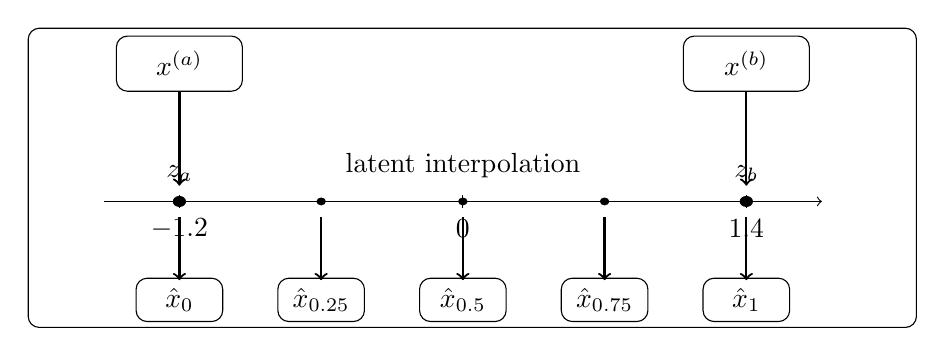
\begin{tikzpicture}[x=1.2cm,y=1cm]
    \draw[rounded corners] (-4.6,-1.6) rectangle (4.8,2.2);
    \draw[->] (-3.8,0) -- (3.8,0);
    \foreach \x/\lab in {-3/-1.2,0/0,3/1.4} {
        \draw (\x,0.08) -- (\x,-0.08);
        \node at (\x,-0.35) {$\lab$};
    }
    \fill (-3,0) circle (0.07);
    \fill (3,0) circle (0.07);
    \fill (-1.5,0) circle (0.05);
    \fill (0,0) circle (0.05);
    \fill (1.5,0) circle (0.05);
    \node at (-3,0.35) {$z_a$};
    \node at (3,0.35) {$z_b$};
    \node at (0,0.45) {latent interpolation};
    \draw[->,thick] (-3,1.4) -- (-3,0.2);
    \draw[->,thick] (3,1.4) -- (3,0.2);
    \node[draw,rounded corners,minimum width=1.6cm,minimum height=0.7cm] at (-3,1.75) {$x^{(a)}$};
    \node[draw,rounded corners,minimum width=1.6cm,minimum height=0.7cm] at (3,1.75) {$x^{(b)}$};

    \draw[->,thick] (-3,-0.2) -- (-3,-1.0);
    \draw[->,thick] (-1.5,-0.2) -- (-1.5,-1.0);
    \draw[->,thick] (0,-0.2) -- (0,-1.0);
    \draw[->,thick] (1.5,-0.2) -- (1.5,-1.0);
    \draw[->,thick] (3,-0.2) -- (3,-1.0);

    \node[draw,rounded corners,minimum width=1.1cm,minimum height=0.55cm] at (-3,-1.25) {$\hat x_0$};
    \node[draw,rounded corners,minimum width=1.1cm,minimum height=0.55cm] at (-1.5,-1.25) {$\hat x_{0.25}$};
    \node[draw,rounded corners,minimum width=1.1cm,minimum height=0.55cm] at (0,-1.25) {$\hat x_{0.5}$};
    \node[draw,rounded corners,minimum width=1.1cm,minimum height=0.55cm] at (1.5,-1.25) {$\hat x_{0.75}$};
    \node[draw,rounded corners,minimum width=1.1cm,minimum height=0.55cm] at (3,-1.25) {$\hat x_1$};
\end{tikzpicture}
\caption{A VAE interpolation sketch. Two examples are encoded into latent points, a line segment is traversed in latent space, and the decoder maps that path back to data space. Smooth interpolation is evidence of learned latent organization, but not proof of semantic disentanglement.}
\label{fig:vaeinterp}
\end{figure}

\subsection*{Case study 3: GAN mode collapse on a toy bimodal target}

A useful way to understand both the power and fragility of adversarial learning is to study a target distribution with two modes.
Consider the one-dimensional target distribution
\[
p_{\mathrm{data}}=\tfrac12\,\delta_{-2}+\tfrac12\,\delta_{2},
\]
which places equal mass near $-2$ and $2$.
Suppose the generator collapses to a single mode and produces only samples near $2$.
Then the model distribution is approximately
\[
p_G\approx \delta_2.
\]

This is a bad model of the true distribution, yet it may still produce individually plausible samples.
That is the pedagogical point.
Adversarial training optimizes distribution matching through a discriminator, but the generator is rewarded through whatever gradient information the current discriminator provides.
If the discriminator is finite-capacity, trained imperfectly, or observed only through stochastic minibatches, the generator may keep exploiting the same successful region instead of covering all modes.

In this toy example, half the target support is missed completely.
The failure is not that the generator cannot produce realistic points.
The failure is that realism and coverage are different notions.
A single sharp mode may look convincing sample by sample while still representing the data distribution poorly.

\begin{figure}[h]
\centering
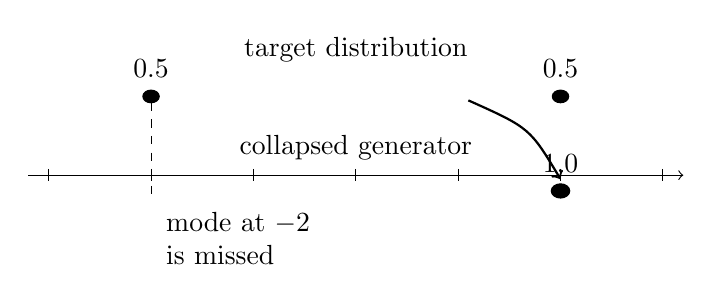
\begin{tikzpicture}[x=1.3cm,y=1cm]
    \draw[->] (-3.2,0) -- (3.2,0);
    \foreach \x in {-3,-2,-1,0,1,2,3} {\draw (\x,0.08) -- (\x,-0.08);}    

    \node at (0,1.6) {target distribution};
    \filldraw (-2,1.0) circle (0.08);
    \filldraw (2,1.0) circle (0.08);
    \node at (-2,1.35) {$0.5$};
    \node at (2,1.35) {$0.5$};

    \node at (0,0.35) {collapsed generator};
    \filldraw (2,-0.2) circle (0.09);
    \node at (2,0.15) {$1.0$};
    \draw[thick,->] (1.1,0.95) .. controls (1.7,0.6) .. (2,-0.05);
    \draw[dashed] (-2,0.92) -- (-2,-0.25);
    \node[align=left] at (-1.15,-0.8) {mode at $-2$\\is missed};
\end{tikzpicture}
\caption{Mode collapse on a bimodal target. The generator produces realistic points near one mode but fails to cover the full data distribution. The example isolates the difference between realism and coverage.}
\label{fig:ganmodecollapse}
\end{figure}

\subsection*{Case study 4: A flow on a two-dimensional density}

Normalizing flows are easiest to understand visually in two dimensions.
Let the base variable be
\[
u=(u_1,u_2)\sim \mathcal{N}(0,I_2),
\]
and define the invertible map
\[
T(u_1,u_2)=\bigl(u_1,\,u_2+0.8\sin(u_1)\bigr).
\]
This is an affine coupling-style transformation: the first coordinate is left unchanged, and the second coordinate is shifted by a function of the first.
The inverse is immediate:
\[
T^{-1}(x_1,x_2)=\bigl(x_1,\,x_2-0.8\sin(x_1)\bigr).
\]
Its Jacobian matrix is
\[
J_T(u)=
\begin{pmatrix}
1 & 0 \\
0.8\cos(u_1) & 1
\end{pmatrix},
\qquad
\det J_T(u)=1.
\]
Therefore the transformed density is
\[
p_X(x_1,x_2)=p_\nu\bigl(x_1,\,x_2-0.8\sin(x_1)\bigr).
\]
The determinant is trivial, but the geometry is not.
Straight contours in the base space become sinusoidally warped contours in data space.
This example shows exactly why flows appeal to mathematically inclined readers:
the model is both visually intuitive and analytically exact.

At the same time, the example exposes the architectural constraint.
The transformation must be invertible and must have a tractable determinant.
These requirements are what make exact likelihood possible, but they also restrict the class of allowable maps.

\begin{figure}[h]
\centering
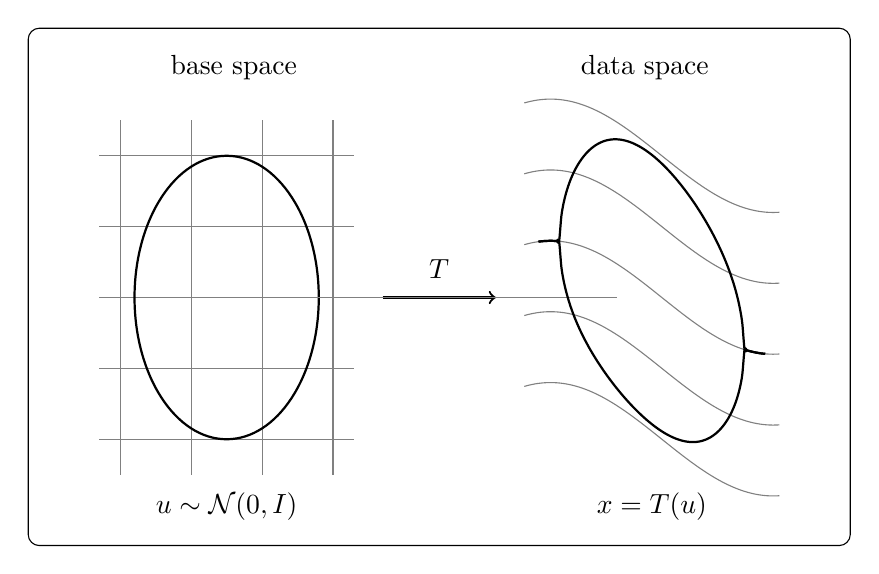
\begin{tikzpicture}[x=0.9cm,y=0.9cm]
    \draw[rounded corners] (-5.8,-3.5) rectangle (5.8,3.8);
    \node at (-2.9,3.25) {base space};
    \node at (2.9,3.25) {data space};
    \draw[->,thick] (-0.8,0) -- (0.8,0);
    \node at (0,0.4) {$T$};

    \foreach \x in {-4.5,-3.5,-2.5,-1.5} {
        \draw[gray] (\x,-2.5) -- (\x,2.5);
    }
    \foreach \y in {-2,-1,0,1,2} {
        \draw[gray] (-4.8,\y) -- (-1.2,\y);
    }
    \draw[thick] (-3,0) ellipse (1.3 and 2.0);
    \node at (-3,-2.95) {$u\sim \mathcal{N}(0,I)$};

    \foreach \x in {1.3,2.3,3.3,4.3} {
        \draw[gray,domain=-2.5:2.5,smooth,samples=50] plot ({\x + 0.0*cos(\x r)},{\x*0 + \x*0});
    }
    \foreach \y in {-2,-1,0,1,2} {
        \draw[gray,domain=1.2:4.8,samples=80,smooth] plot (\x,{\y + 0.8*sin(\x r)});
    }
    \draw[thick,domain=1.4:4.6,samples=100,smooth] plot (\x,{1.9*sqrt(max(0,1-((\x-3)/1.3)^2)) + 0.8*sin(\x r)});
    \draw[thick,domain=1.4:4.6,samples=100,smooth] plot (\x,{-1.9*sqrt(max(0,1-((\x-3)/1.3)^2)) + 0.8*sin(\x r)});
    \node at (3,-2.95) {$x=T(u)$};
\end{tikzpicture}
\caption{A two-dimensional flow warps a simple base density into a curved target density by an invertible transport map. Because the map is explicit and invertible, both sampling and density evaluation remain exact.}
\label{fig:flowwarping}
\end{figure}

\subsection*{Case study 5: Diffusion denoising trajectory on a toy distribution}

Diffusion models are easiest to grasp when viewed as progressive correction rather than single-shot sampling.
Take a one-dimensional toy distribution concentrated near two modes, say near $-2$ and $2$.
A forward corruption process repeatedly adds Gaussian noise until the distribution becomes approximately normal around $0$.
The reverse process then learns to nudge a noisy point back toward one of the data-supported regions.

A tiny numerical sketch makes this concrete.
Suppose the reverse model starts from $x_4=0.3$ and at each step predicts a denoised mean that moves toward the positive mode:
\[
\hat x_3=0.9,
\qquad
\hat x_2=1.4,
\qquad
\hat x_1=1.8,
\qquad
\hat x_0=2.0.
\]
This is not meant to mimic a real trained network exactly.
It is a pedagogical summary of what the learned reverse chain does: each step removes some uncertainty while preserving enough randomness that different runs can end at different supported regions of the data distribution.

The crucial contrast with GANs is that diffusion does not attempt to jump directly from noise to data in one step.
The crucial contrast with flows is that the path need not be invertible in one shot.
The crucial contrast with VAEs is that the hidden variables are not summarized by one global latent code, but by a whole sequence of refinement states.

\begin{figure}[h]
\centering
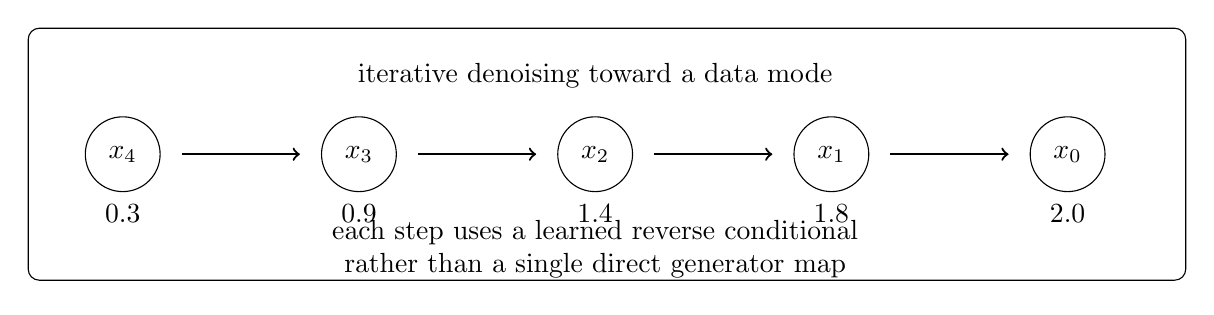
\begin{tikzpicture}[x=1.5cm,y=1cm]
    \draw[rounded corners] (-0.8,-1.6) rectangle (9.0,1.6);
    \node[draw,circle,minimum size=0.95cm] (x4) at (0,0) {$x_4$};
    \node[draw,circle,minimum size=0.95cm] (x3) at (2,0) {$x_3$};
    \node[draw,circle,minimum size=0.95cm] (x2) at (4,0) {$x_2$};
    \node[draw,circle,minimum size=0.95cm] (x1) at (6,0) {$x_1$};
    \node[draw,circle,minimum size=0.95cm] (x0) at (8,0) {$x_0$};
    \draw[->,thick] (0.5,0) -- (1.5,0);
    \draw[->,thick] (2.5,0) -- (3.5,0);
    \draw[->,thick] (4.5,0) -- (5.5,0);
    \draw[->,thick] (6.5,0) -- (7.5,0);
    \node at (0,-0.75) {$0.3$};
    \node at (2,-0.75) {$0.9$};
    \node at (4,-0.75) {$1.4$};
    \node at (6,-0.75) {$1.8$};
    \node at (8,-0.75) {$2.0$};
    \node at (4,1.0) {iterative denoising toward a data mode};
    \node[align=center] at (4,-1.2) {each step uses a learned reverse conditional\\rather than a single direct generator map};
\end{tikzpicture}
\caption{A toy diffusion denoising trajectory. Starting from a noisy sample, the reverse process repeatedly refines the state toward a data-supported region. The picture emphasizes iterative correction rather than exact numerical realism.}
\label{fig:difftrajectory}
\end{figure}

\subsection*{One family of toy problems, many modeling viewpoints}

We can now compare the paradigms through the same pedagogical lens.
The Gaussian mixture explains multimodality through an explicit latent assignment variable.
The VAE explains it through a continuous latent code and a decoder.
The GAN tries to match the target distribution through adversarial training, but can fail by concentrating on only one of several modes.
The flow transports a simple base distribution into a more complex one through an invertible map.
The diffusion model constructs generation as a sequence of denoising refinements.

This is the central lesson of the section.
The paradigms are not merely different software stacks.
They embody different answers to the question ``how should a complicated data distribution be represented?''
A mathematically inclined reader should notice that the hidden variable, the training objective, and the generative mechanism are coupled differently in each family.

\begin{table}[h]
\centering
\small
\renewcommand{\arraystretch}{1.2}
\begin{tabular}{|p{2.2cm}|p{3.6cm}|p{4.2cm}|}
\hline
\textbf{Paradigm} & \textbf{What the toy example highlights} & \textbf{Main caution revealed by the toy example} \\
\hline
Gaussian mixture / EM & Hidden assignments can turn a difficult marginal-likelihood problem into alternating weighted updates. & Local optima and component assumptions matter; the latent variable is discrete and model-specific. \\
\hline
VAE & Continuous latent coordinates can organize variation and support interpolation. & Interpolation quality depends on decoder behavior and actual latent usage. \\
\hline
GAN & High local realism does not guarantee full distributional coverage. & Mode collapse can hide behind plausible samples. \\
\hline
Flow & Exact density modeling can be visualized as invertible transport of probability mass. & Invertibility and tractable Jacobians constrain the architecture. \\
\hline
Diffusion & Generation can be understood as repeated denoising rather than one-shot synthesis. & Sampling is iterative and therefore computationally expensive. \\
\hline
\end{tabular}
\caption{A comparative summary of what each worked example teaches.}
\label{tab:workedgensummary}
\end{table}

\subsection*{What to remember}

\begin{itemize}
    \item Low-dimensional worked examples reveal structural differences among generative paradigms that are easy to miss in large-scale applications.
    \item EM explains multimodality through latent assignments; VAEs through continuous latent coordinates; GANs through adversarial distribution matching; flows through invertible transport; diffusion through iterative denoising.
    \item A visually convincing sample is not the same thing as good density coverage.
    \item Interpolation, transport, and denoising pictures are useful diagnostics, but they should be interpreted carefully rather than treated as proofs of deep understanding.
\end{itemize}

\subsection*{Common confusion}

\begin{itemize}
    \item A VAE interpolation path is not guaranteed to remain on the true data manifold.
    \item A GAN that produces sharp samples may still model the data distribution poorly if it misses modes.
    \item A flow picture may look simple only because the low-dimensional example hides the architectural burden of invertibility in higher dimensions.
    \item A diffusion trajectory is stochastic refinement, not deterministic decoding from a single latent code.
\end{itemize}

\subsection*{Exercises}

\begin{enumerate}
    \item Recompute the first EM iteration in the Gaussian-mixture example with initial means $\mu_1^{(0)}=-0.5$ and $\mu_2^{(0)}=0.5$. How do the responsibilities and updated means change?
    \item In the VAE interpolation example, suppose the decoder mean is $\mathbb{E}[x\mid z]=z^3$ instead of $2z$. Compute the decoded values along the same interpolation path and explain how nonlinearity changes the interpretation.
    \item Construct a three-mode target distribution for which a GAN-like generator that covers only two modes would still produce visually plausible samples. Why is this failure hard to see from isolated samples alone?
    \item For the flow example, verify explicitly that $\det J_T(u)=1$ and compute $p_X(0,1)$ in terms of the standard Gaussian density.
    \item Consider a toy diffusion process with three reverse steps and predicted means $0.1\to 0.7\to 1.3\to 2.0$. Explain which parts of this trajectory are deterministic and which parts would be stochastic in an actual diffusion sampler.
    \item Take the same one-dimensional bimodal target and explain, in one paragraph each, how a Gaussian mixture, a VAE, a GAN, a flow, and a diffusion model would represent it.
\end{enumerate}

\subsection*{Notes and references}

These worked examples are deliberately elementary, but they mirror the conceptual structure of the major paradigms.
The EM walk-through reflects the classical latent-variable literature for Gaussian mixtures and incomplete-data likelihood.
The interpolation sketch is the simplest visual diagnostic for latent-variable autoencoders.
The mode-collapse example abstracts a major theme from the GAN literature: adversarial realism does not automatically imply full support coverage.
The flow example reflects the transport viewpoint of invertible density models.
The denoising trajectory is the simplest low-dimensional analogue of the iterative sampling picture used in modern diffusion models.

For a reader studying the literature, the right habit is to ask, in each case, what is mathematically exact, what is an approximation, and what is an empirical visualization meant only to build intuition.
